\paragraph{Démonstration}
	\begin{itemize}
		\item Une masse m soumis aux forces $F_c$
		\item PFD : $\sum_i \vec{F_i} = m\vec{a}$
		\item Sur une seule dimension : \[\left\{\begin{array}{rcl}
			\vec{v} &=& \dot{x} \cdot \vec{i} \\
						\vec{F_i} &=& F_{ix} \vec{i}
		\end{array}\right.\]
	\end{itemize}
		\[\begin{array}{rclr}
			m\ddot{x} \vec{i} &=& \sum_i F_{ix} \vec{i} \\
			(m\ddot{x}\vec{i})(\dot{x}\vec{i}) &=& (\sum_i F_{ix} \vec{i})(\dot{x}\vec{i}) \\
			m\ddot{x}\dot{x} &=& \sum_i F_{ix} \cdot \dot{x} \\
			m(\frac{d}{dt}(\dot{x(t)}))^2 \frac{1}{2} &=& \sum_i F_{ix} \cdot \dot{x} \\
			\int_A^B m(\frac{d}{dt}(\dot{x(t)}))^2 \frac{1}{2} dt &=& \int_A^B \sum_i F_{ix} dx & \dot{x} = \frac{dx}{dt} \\
				\frac{1}{2} m [\dot{x(t)}^2]_A^B &=& \int_A^B \sum_i F_{ix} \vec{i}dx = \int_A^B \sum_i dW(F_{ix}\vec{i}) dx \\
			\text{D'où } \frac{1}{2}m [\dot{x}^2]^B_A = \sum_i W_{A \to B} (\vec{F_i})
		\end{array}\]

\paragraph{Exemple d'utilisation}
	\begin{wrapfigure}[5]{r}{0pt}
		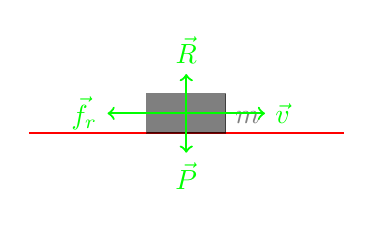
\begin{tikzpicture}
			\draw[thick, red] (-2, 0) -- (2, 0);
			\draw[fill=black, opacity = 0.5] (-0.5, 0.5) rectangle (0.5, 0) node [above right] {$m$};
			\draw[->, thick, green] (0, 0.25) --+ (1, 0) node [right] {$\vec{v}$};
			\draw[->, thick, green] (0, 0.25) --+ (-1, 0) node [left] {$\vec{f_r}$};
			\draw[->, thick, green] (0, 0.25) --+ (0, 0.5) node [above] {$\vec{R}$};
			\draw[->, thick, green] (0, 0.25) --+ (0, -0.5) node [below] {$\vec{P}$};
		\end{tikzpicture}
	\end{wrapfigure}

	Quelle est la distance parcourue par m avant de s'arrêter ?

	\[\left\{\begin{array}{c}
		\text{Soit une masse m de vitesse initiale } \vec{v_0} \\
		\text{Force de frottement solide } \\
		\vec{dl} = \vec{i}\cdot x \text{ le déplacement élémentaire } \\
		\vec{P} + \vec{R} = \vec{0} \\
		\delta E_c = \sum_iW(\vec{F_i})\\
		\sum_iW(\vec{F_i}) = W(\vec{P}) + W(\vec{R}) + W(\vec{f}) \\
	\end{array}\right.\]

	\[\left.\begin{array}{rcl}
			W(\vec{P}) &=& 0 \\
			W(\vec{R}) &=& 0 
	\end{array}\right\}
	\text{Car } \vec{P} \text{ et } \vec{R} \text{ sont perpendiculaire de } \vec{v}\]


	\[\begin{array}{rcl}
			W_{A \to B} (\vec{f}) &=& \int_A^B \vec{f}\vec{dl} = \int_A^B (||\vec{f}||\cdot \vec{i}) (dx \vec{i}) \\
			||\vec{f} &=& k_c ||\vec{R}|| = k_c ||m\vec{g}|| \\
			W_{A \to B} (\vec{f}) &=& \int_A^B -(k_c mg)\cdot dx \\
					  &=& -k_c mg[x]^B_A \\
			\delta E_c &=& \frac{1}{2} m [v_B^2 - v^2_A] = -k_c mg[x_B - x_A]
	\end{array}\]

	\[\left\{\begin{array}{rcl}
		x_A &=& \text{ point de départ } v = v_0 \\
		x_B &=& \text{ point d'arriver de la masse} v = 0 
		\end{array}\right.\]

		Donc
		\[\begin{array}{rcl}
				-\frac{1}{2} m v_0^2 &=& -k_c mg(d_{AB}) \\
				d_{AB} &=& \frac{mv_0^2}{2gk_cm} = \frac{v_0^2}{2gk_c}
		\end{array}\]
	

		\paragraph{Autre forme de théorème $E_c$}
		\[\begin{array}{rclr}
			E_c &=& W_{AB} (\vec{F}) \Rightarrow dE_c = dW(\vec{f}) \\
				\frac{dE_c}{dt} &=& \frac{dW(\vec{f})}{dt} \Rightarrow \frac{dE_c}{dt} = \frac{\vec{F}\vec{dl}}{dt} \\
				\frac{dE_c}{dt} &=& \vec{F}\cdot \frac{\vec{dl}}{dt} = \vec{F}\vec{v} \\
				P &=& \frac{dE_c}{dt} = \vec{F}\cdot \vec{v} & \text{ Puissance développée par } \vec{F} \\
				{[P]} &=& ML^2 T^{-3}
		\end{array}\]


\section{Forces conservatives}
\subsection{Energie Potentielle}

\paragraph{Définition} Une force est conservative si elle ne dépend que de la position des points d'arrivée de de départ, \ul{et} son travaille ne dépend pas du chemin suivi entre 2 points A et B pour tout \ul{A et B}.

\paragraph{Exemple}

Force rappel d'un ressort : 

\begin{itemize}
	\item $\vec{F} = -kx\vec{i}$
\end{itemize}
\[\begin{array}{rcl}
		W_{AB} &=& \int_A^B \vec{F}\vec{dl} = \int_A^B (-kx\vec{i}) dx\vec{i} \\
		W_{A \to B} &=& [-\frac{1}{2}kx^2]^B_A \\
			   &=& \frac{1}{2}k[x^2_A - x^2_B] \\
\text{Si on passe par c } W_{A\to B} &=& W_{A \to C} + W_{C \to B} \\
			   &=& \frac{1}{2}k(x^2_A - x^2_C) + \frac{1}{2}k(x^2_C-x^2_B) \\
			   &=& \frac{1}{2}k(x^2_A - x^2_B)
\end{array}\]o
La force de rappel d'un ressort est conservative.

\subsection{Force de frottement fluide}

\[\begin{array}{rclr}
		\vec{f} &=& -\lambda \vec{v} \\
		W_{A \to B}(\vec{f}) &=& \int_A^B \vec{f}\vec{dl} \\
			  &=& \int_A^B(-\lambda \vec{v}) \vec{dl} \\
			   &=& -\lambda \int_A^B(\dot{x})(\vec{i})(dx\vec{i})  \\
			&=& -\lambda \int_A^B (\frac{dx}{dt}) dx  \\
			&=& -\lambda \int_A^B(\ddot{x^2} dt & dx = \frac{dx}{dt}dt
\end{array}\]

La force de frottement n'est donc pas conservatrice car dépend du temps.

\subsection{Travail du poids}

\[\begin{array}{rcl}
		W_{A \to B} &=& \int_A^B \vec{P}\cdot \vec{dl} \\
											   &=& \int_A^B (||m\vec{g}||)\vec{k}\cdot\vec{dl} = ||m\vec{g}||\int_A^B \vec{k}\vec{dl} = ||m\vec{g}||\int_A^B ||\vec{dl}||\cdot \cos(\Theta)
\end{array}\]

\subsection{Energie potentielle}

Quand une force est conservative, il existe une fonction $E_p$ tel que : \[W_{A \to B} (\vec{F}) = E_p(A) - E_p(B)\] pour tout A, B.
Sur une chemin rectiligne $AB // O_x$

\[W_{AB}(\vec{F}) = E_p(x_A) - E_p(x_B)\]

Dans le cas globale : $\overrightarrow{AB}(x, y, z)$ : 
\[\begin{array}{rcl}
	W_{AB}(\vec{F}) = E_p(x_A, y_A, z_A) - E_p(x_B, y_B, z_B) 
\end{array}\]

Relation $\vec{F}$ et $E_p$

\[\begin{array}{rcl}
	W_{A \to B}(\vec{F}) &=& \int_A^B \vec{F}\cdot \vec{dl} = E_p^{(A)} - E_p^{(B)}
\end{array}\]

Sur chaque direction, $W_{A \to B} = \int_A^B F_{x, y, z} d(x, y, z) = E_p (x, y, z)_A - E_p(x, y, z)_B$ ~\\
\[\text{Donc }\left\{\begin{array}{rcl}
			F_x dx &=& -dE_p(x)|^B_A \\
			F_ydy &=& -dE_p(y)|^B_A \end{array}\right.\]

			\[\left\{\begin{array}{rcl}
			F_x &=& -\frac{dE_p}{dx} \\
						F_y &=& -\frac{dE_p}{dy} \\
						F_z &=& -\frac{dE_p}{dz} \\
				\end{array}\right.\]

	On dit que $\vec{F}$ dérive de $E_p$, avec $E_p$ l'énergie potentielle.

\paragraph{En 3D} \[dW = \vec{F}\vec{dl} = -dE_p\]

Ou $\vec{F} = -(\frac{dE_p}{dx}\vec{i} + \frac{dE_p}{dy}\vec{j} + \frac{dE_p}{dz}\vec{k})$ ~\\
À l'inverse, \[\begin{array}{rcl}
		dE_p(x, y, z) &=& F_xdx + Fy dy + F_z dz \\
												 &=& \overrightarrow{grad}(E_p)
\end{array}\]

$E_p$ est connu à une constante près.
